\documentclass[a4paper,12pt]{article}
\usepackage{float, graphicx}
\graphicspath{ {./Images/} }
\usepackage{amsfonts, url}
\usepackage[margin=0.984252in]{geometry}
\urlstyle{same}

\begin{document}
    \renewcommand{\refname}{Bibliography}

    \begin{center}
        \huge
        \textbf{Kids Emotions Detection}
        \normalsize
    \end{center}

    \section*{Team}
    \begin{itemize}
        \item Tigau-Almasan Alexandra (258/2)
        \item Gorgos Andreea (258/1)
        \item Corman Robert (258/1)
    \end{itemize}

    \section*{Data}

    \begin{itemize}
        \item \url{https://www.childstudycenter-rutgers.com/the-child-affective-facial-expression-se}
    \end{itemize}

    \section*{Problem description}
    \paragraph{}
    Because we want to know which was the kids emotion when they were trying to use technology/applications,
    based on photos took while they were playing with the app we are trying to discover their emotions. This 
    emotions are identified in order to have an objective way of analysing their emotions while interacting with the system. 

    \section*{Related work and useful tools}

    \begin{itemize}
        \item THE BEST OF 2019 - \url{https://azure.microsoft.com/en-us/services/cognitive-services/face/}
        \begin{itemize}
            \item dataset: \url{https://megapixels.cc/datasets/msceleb/}
            \item results: AFEW - 45\%; SAVEE - 56\%; RAVDESS - 39\%;
            \item algorithm: CNN
            \item Facial expressions: Neutral, Anger, Happiness, Anger, Surprise, Sadness, Disgust, Fear
        \end{itemize}
        \item VIDEO - \url{https://www.youtube.com/watch?v=CVClHLwv-4I&fbclid=IwAR2o_mLoZHYXzg532OVW-eqYO4qa_rmRQPgUC9uReE9xVkpGkHoTQuagnQ4}
        \item \url{https://blog.rapidapi.com/top-facial-recognition-apis/?fbclid=IwAR374W-397MFM4vsFaL6d1QXiu7HJu7kFDHspFhCHc5wZ11gk3Elm4GUvec}       
        \item  Emotion Detection Algorithm Using Frontal Face Image \url{https://www.researchgate.net/publication/228870902_Emotion_Detection_Algorithm_Using_Frontal_Face_Image}
        \begin{itemize}
            \item dataset: 20 men and 10 women, under same
            position and slightly different illumination condition, 5 facial
            images representing 5 different emotions
            person.
            \item results: 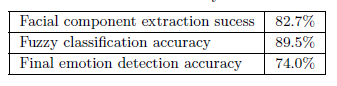
\includegraphics[]{emotion-accuracy.png}
            \item algorithm: 3 stages: image precessing stage, facial feature extrac-
            tion stage, and emotion detection stage
            \item Facial expressions: happy, sad, disgust, surprise,
            and angry
        \end{itemize}
        \item Image-based emotion recognition using evolutionary algorithms \url{https://www.sciencedirect.com/science/article/abs/pii/S2212683X18300185}
        \item  A hybrid approach \url{https://pdfs.semanticscholar.org/d551/0e0d8bdf245d6c8e7cb49ba287f7dca235a1.pdf}
        \begin{itemize}
            \item dataset: JAFFE
            \item results: 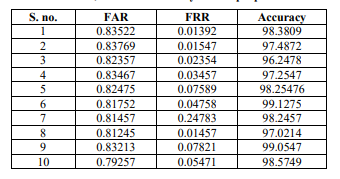
\includegraphics[]{hybrid-approach.png}
            \item algorithm: 5 steps: face acquisition, pre-processing, face detection, feature extraction, classification
            \item Facial expressions: Angry, Disgusted, Fear, Happy, Sad and Surprised
        \end{itemize}
        \item  High-performance and lightweight real-time deep face emotion recognition \url{https://www.researchgate.net/publication/319413472_High-performance_and_lightweight_real-time_deep_face_emotion_recognition}
        \begin{itemize}
            \item dataset: AFEW, FER, Cohn-Kanade
            \item results: AFEW - 32, 6\% ; FER - 70\% 
            \item algorithm: CNN
            \item Facial expressions: Anger, Disgust, Fear, Joy, Neutrality, Sadness
            and Surprise
        \end{itemize}
        \item TOP 10 - \url{https://www.luxand.com/facesdk/?gclid=Cj0KCQjw84XtBRDWARIsAAU1aM3rgi25ZV8vilOf9qKagvkr6GeasvTAxb-NpAKdNSuTBvMC38q6XhwaAu--EALw_wcB}
    \end{itemize}

    \section*{Objectives}
    \begin{itemize}
        \item Choose a database
        \item Try out more face recognition sdks
        \item Choose two sdks from the list above
        \item Use those 2 and make a comparison
        \item Create an app which will use the 2 sdks in real-time/recognised by an image
    \end{itemize}

    \section*{The app's use-cases}

    \paragraph{}
    open app -\textgreater\textvisiblespace
    choose algorithm to use -\textgreater\textvisiblespace
    choose a photo -\textgreater\textvisiblespace
    analyze the face -\textgreater\textvisiblespace
    display the emotion and the accuracy -\textgreater\textvisiblespace
    button for retry

    \begin{thebibliography}{9}
        
    \end{thebibliography}
\end{document}